\documentclass[]{article}

\usepackage{graphicx}

%in order to avoid vertical spacing between list items
\usepackage{enumitem}
\usepackage{caption}
%placeholder shortcut
\newcommand{\ph}[1]{{\textless}#1{\textgreater}}

% no indentations for new paragraphs
\setlength{\parindent}{0pt}

\begin{document}
	\begin{titlepage}
		\centering
		\vspace*{\fill}
		
		\vspace*{0.5cm}
		
		\huge\bfseries
		SPSS BatchProcessor
		
		\vspace*{0.5cm}

		\small
		Psychologische Diagnostik. Differentielle Psychologie und Persönlichkeitspsychologie\\
		CAU Kiel
		
		\vspace*{\fill}
	\end{titlepage}
	
	

\tableofcontents

\section{Introduction}

The \textit{SPSS BatchProcessor} is a Python tool to batch-process large quantities of files. It processes a given set of files, extracting specified information from each file and executing a given SPSS file on each data file.
Even though it is called \textit{SPSS BatchProcessor}, it can run both \textit{SPSS} as well as \textit{PSPP}.  

For SPSS, it relies on the Python interface provided by SPSS and delegates commands line-wise to SPSS; for PSPP, it relies on PSPP's command line interface.

In the following we will assume that you store one subject per file. This is a convenient way to organize the data, however you are free to use any other form of organization as well. We will work with subject files of the pattern
\begin{verbatim}
pb_123_condition.txt
\end{verbatim}
where ''123'' is a unique identifier of the subject and ''condition'' refers to the conditions of the underlying experiment. 

For instance, let's assume that we conduct an experiment which employs a cooperation/non-cooperation scheme (e.g. ''prisoner's dilemma''). In this situation, ''fair/unfair'' might be a reasonable categorization for situations the subject is presented with, each encoding the behavior of the computer. 

The BatchProcessor performs the following steps for a each file in a given set:
\begin{itemize}[noitemsep]
	\item extract information from input file
	\item load SPSS syntax file. Substitute placeholders in said file
	\item delegate execution of file to SPSS
\end{itemize}

\subsection{Installation}
The BatchProcessor is essentially a Python script which is executed using the Python environment shipped with every SPSS installation. 

Installation is quite straightforward; the uncompressed BatchProcessor directory may be placed in an arbitrary directory, then we need to specify the way of execution. To that end, it is sufficient to create a link (as in Windows file link) to the Python interpreter as follows:
\begin{verbatim}
"C:\Program Files\IBM\SPSS\Statistics\24\Python\python.exe"
 "C:\[\]...]\SPSSToolbox\batchProcessor\batchProcessor.py"
\end{verbatim}
\begin{small}
	Please note: no newline in between - just inserted to fit into this document
\end{small}

The version number of SPSS, here ''24'' needs to be replaced by your respective version; alternatively feel free to specify an arbitrary installation directory if yours happens to differ from the default one. 

\subsection{Typical Workflow}
Once a processing stage has been developed and configured, the workflow will typically be as follows:
\begin{itemize}[noitemsep]
	\item Load predefined configuration for processing stage
	\item select input files
	\item hit ''Run''
\end{itemize}

\subsection{Interface}
When the program starts up, the following interface will be shown:\\

\begin{minipage}{\linewidth}% to keep image and caption on one page
	\makebox[\linewidth]{%        to center the image
		\fbox{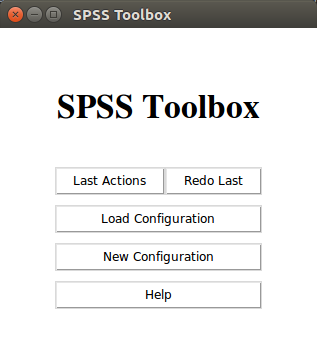
\includegraphics[width=0.5\textwidth]{img/mainWindow.png}}}
	\captionof{figure}{Main Window presenting options}
\end{minipage}

The main window presents a variety of options to access \textit{configurations}; however, this interface is not pertinent to the processing itself. All of those options redirect the operator to the following interface:

\begin{minipage}{\linewidth}% to keep image and caption on one page
	\makebox[\linewidth]{%        to center the image
		\fbox{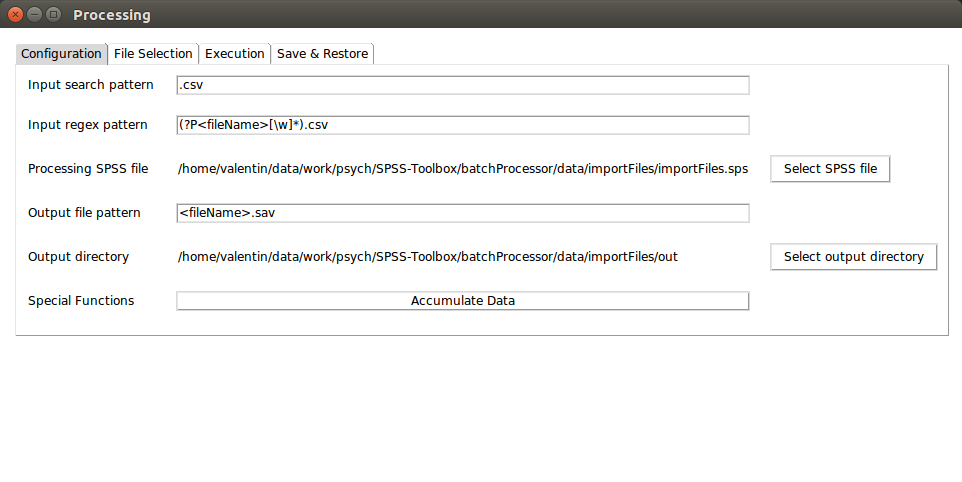
\includegraphics[width=1.3\textwidth]{img/general_interface.png}}}
		\captionof{figure}{Interface upon startup with default settings}
\end{minipage}

\begin{enumerate}
	\item \textbf{Configuration}
\begin{enumerate}
	\item \textbf{Input search pattern:} A search pattern for the input files to select. When selecting files using ''Select input files'', only files matching the input search pattern will be displayed. \\
	
	Note that this comes in handy when \textit{filtering} subject files with respect to conditions. For instance, you might specify ''\_unfair.txt'' to process only subjects for a certain condition. You can also specify a filter like ''pb\_*\_condition1\_*\_condition2.txt'' if you wish to filter for several conditions which might or might not be contiguous in the file name. ''*'' is a pattern which matches \textit{all} characters. 
	
	Please note that the pattern is \textit{not} a full-fledged REGEX pattern, but rather a GLOB pattern. In a nutshell, you should only use ''*'' as a wildcard pattern. 
	
	\item \textbf{Select Dir:} Select an entire directory to process. This will select \textit{all} files in said directory without considering the \textit{Input Search Pattern}. There are mainly two reasons for using this method:
	
	\begin{itemize}
		\item You have a dedicated directory for each stage of your processing pipeline
		\item You have so many files that Windows does not let you select them manually. 
	\end{itemize}

	\item \textbf{Input regex pattern:} Pattern to extract information from the filename; this information can then be used inside the SPSS syntax for processing. Please refer to the dedicated chapter. 
	
	\item \textbf{Processing SPSS file:} A regular SPSS file to use for processing. The SPSS file will be executed \textit{individually} for every selected input file. Please refer to the dedicated chapter on specifics like placeholders. 
	
	\item \textbf{Output file pattern:} Specifies how to populate the placeholder ''\ph{OUTPUTFILE}'' in the SPSS syntax. If you do not use said placeholder, you can just provide a dummy value like ''dummy.sps''. 
	
	\item \textbf{Output directory:} Used to construct '\ph{OUTPUTFILE}''. Apart from that, it is directly available as ''\ph{OUTPUTDIR}'' in the syntax. 
		
	\item \textbf{Accumulate Data:} This function aggregates/accumulates multiple files into a single file. It comes in handy when grouping subjects by conditions; for instance, the operator may perform an analysis over all subjects with the condition ``fair''. Afterwards, he may draw conclusions by comparing characteristics of this group with groups of other conditions. 
	
	This function will is built-in and will automatically disable features and configuration options irrelevant to this operation. The final file is called ``accumulate.sav'' and is stored in the specified output directory. 
\end{enumerate}
	\item \textbf{Save and Restore}
	\begin{itemize}
	\item \textbf{Load/Save config:} Saves the input search pattern, the input regex pattern, spss file, file output pattern and output directory to a configuration file of your choice. It does \textit{not} save the selected input files. When loading input files, the loaded settings are presented to the operator. 
	
	This feature is meant to save a configuration for each stage of your processing; the settings for each stage can then just be loaded upon execution and shared with your colleagues. 
	
\end{itemize}

	\item \textbf{Execution}
\begin{itemize}
	\item  \textbf{Simulate:} When activated, the processing is only simulated and \textit{not} passed to SPSS. Instead, processing of the \textit{very first selected file} is simulated and the resulting placeholders as well as commands are presented to the operator. This is a useful tool for debugging. 
	
	\item \textbf{Run:} Starts the processing. The progress bar will keep track of the progress, furthermore an estimate of the remaining time for processing is given. This can be leveraged to replenish depleted levels of caffeine.  
	When processing is finished, a summary is displayed. 
	
	{\small It is possible to use distribute the work to multiple processors; however you will need to make those changes in the code itself. }
\end{itemize}

\end{enumerate}


\section{Processing}
\subsection{Placeholders}
Placeholders are strings of the form ''\ph{placeholderName}'' which are replaced with suitable information. They can be used in the \textit{SPSS syntax} as well as in the \textit{output file pattern}. Placeholders in the SPSS file syntax which were not provided\footnote{by either the \textit{input file pattern} or \textit{manually defined placeholders} in the configuration file} will simply be ignored; in the output file pattern, however, undefined placeholders will result in an error. 

\subsubsection{Usage}
Placeholders of the form ''\ph{placeholderName}'' will be replaced at the location where they are found. Placeholders may contain arbitrary strings except for ''\textless'' and ''\textgreater''. 

\subsubsection{Definition}
Placeholders can either be defined in the configuration file (which makes them static), or they can be extracted from the file name. Configuration files can be edited with any text editor (such as notepad) and will look as follows:
\begin{verbatim}
{
"defaultConfigDir": ".", 
"defaultInputDir": ".", 
"defaultOutDir": ".", 
"defaultSPSSDir": ".", 
"inputRegexPattern": "(?P<fileName>[\\w]*).txt", 
"inputSearchPattern": ".txt", 
"outputDir": "none selected", 
"outputFilePattern": "<fileName>.sav", 
"placeholders": {
    "DUMMY": "DUMMY", 
    "INFILE": "", 
    "OUTPUTFILE": ""
},
"programVersion": 0.8, 
"spssFile": "none selected"
}
\end{verbatim}
Feel free to add new placeholders in the respective section; be sure to separate them from other placeholders using a '','' and wrapping both the name and the value with quotation marks, separating those two with '':''. The file is in \textit{JSON} syntax, which makes it easily accessible using a variety of tools while still being readable and editable by humans. 

Please note that there are a number of \textit{predefined placeholders} which will be \textit{overwritten} when specified manually.

\subsubsection{Predefined placeholders}
The following placeholders are automatically provided to the SPSS syntax:
\begin{itemize}[noitemsep]
	\item \textbf{INFILE:} The full path including the file name of the input file
	\item \textbf{INPUTDIR:} The input directory of the input file
	\item \textbf{OUTPUTFILE:} The full path including the file name
	\item \textbf{OUTPUTDIR:} The output directory 
	\item \textbf{fileName:} Just the file name of the input file \textit{without the full path} (as opposed to \textit{INFILE})
\end{itemize}

Additional (static) placeholders may be defined in the configuration file. 
Please note that there is no need to have only \textit{one} output file (which would then be composed by  means of ''\ph{OUTPUTFILE}''. Please note that you can literally just use the pattern for the output file directly in the SPSS syntax. In particular, you can produce several output files using the very same SPSS syntax. 
If you choose to ignore the output file pattern from the interface, please use a dummy placeholder like ''dummy'' to let people know you don't actually use that field.  


\subsection{Input file pattern}
The \textit{input file pattern} is a \textit{REGEX} expression which defines the information to be extracted from each input file. As such, the input file pattern \textit{must} match each and every input file. Should the pattern not match any file, an error will be thrown. 

Placeholders are defined in terms of \textit{named groups}. As there is an abundance of documentation online, we will just provide a short treatment at this point. 
Named groups are of the following form:
\begin{verbatim}
(?P<groupName>[characterSet]*)
\end{verbatim}
where \textit{groupName} is the name of the placeholder to define and \textit{characterSet} defines which characters this group may or may not use. A reasonable choice, encompassing all letters, whitespaces and numbers, is 
\begin{verbatim}
(?P<groupName>[\w]*)
\end{verbatim}
You can define an arbitrary number of named groups. 

For the sample file pattern
\begin{verbatim}
''pb_*_condition1_*_condition2.txt''
\end{verbatim}
we could define the following pattern:
\begin{verbatim}
pb_*_(?P<condition1>[\w]*)_*_(?P<condition2>[\w]*).txt
\end{verbatim}
which will result in the placeholders ''\ph{condition1}'' as well as ''\ph{condition2}'' being present in the SPSS file. 

Please note that any part which is not a part of any named group will simply be ignored. That is true, for instance, for the ''*'' placeholder between ''pb'' and the ''\ph{condition1}'' in the aforementioned example. 

Furthermore, the \textit{predefined placeholders} are always available, regardless of how you choose to design your input pattern.


\section{Debugging}
\begin{minipage}{\linewidth}% to keep image and caption on one page
	\makebox[\linewidth]{%        to center the image
		\fbox{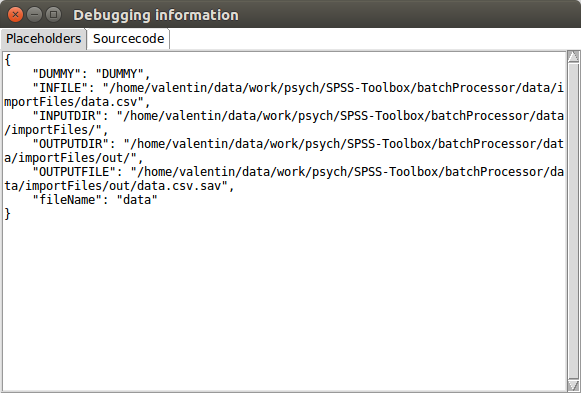
\includegraphics[width=1\textwidth]{img/debugging_interface.png}}}
	\captionof{figure}{Debugging output in simulation mode}
\end{minipage}

When using the \textit{Simulation} mode, processing of the very first selected file will be simulated and the results will be shown as above. You can inspect the placeholders which are used as well as the sourcecode which would be passed to SPSS as-is. When SPSS errors occur, you can paste the syntax into SPSS and continue from there, taking advantage of its built-in debugging features. 

\begin{minipage}{\linewidth}% to keep image and caption on one page
	\makebox[\linewidth]{%        to center the image
		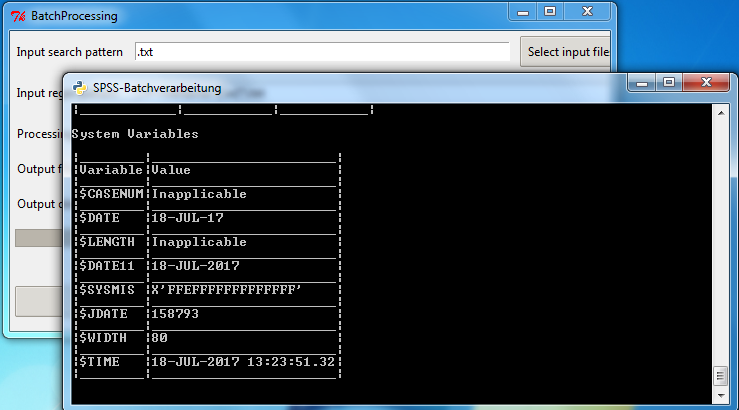
\includegraphics[width=1.3\textwidth]{img/debugging_console.png}}
	\captionof{figure}{Processing console output}
\end{minipage}
Apart from this feature, a second console window will pop up during processing. This window logs the process' every action. You can track the commands being sent to SPSS as well as SPSS's output. If errors occur, the program will halt and you can find the error message in this window. Please note that the error message of SPSS will be interspersed with feedback from the SPSS BatchProcessor as errors cascade down to the BatchProcessor. 


\end{document}          
